\documentclass[../main.tex]{subfiles}
\graphicspath{{../image/}{../figure/}}
\begin{document}

\chapter{变分法}\label{appendix:b-变分法}

我们可以将函数 $y(x)$ 视为如下运算：对于任何输入值 $x$，返回输出值 $y$。同样，我们也可以将\textbf{泛函}（functional）$F[y]$ 视为接收函数 $y(x)$ 并返回输出值 $F$ 的运算。泛函的一个示例是在二维平面上计算绘制的曲线的长度，其中曲线的路径是由一个函数定义的。在机器学习中，一个广泛使用的泛函是连续变量 $x$ 的熵 $H[x]$。对于任意选择的概率密度函数 $p(x)$，它都会返回一个标量值以表示该密度下 $x$ 的熵。因此，$p(x)$ 的熵也可以类似地写作 $H[p]$。

传统微积分中的一个常见问题，就是找到一个 $x$ 值以使函数 $y(x)$ 最大化（或最小化）。类似地，在\textbf{变分法}（calculus of variations）中，我们也要寻求一个函数 $y(x)$，该函数能使泛函 $F[y]$ 最大化（或最小化）。也就是说，在所有可能的函数中，我们希望找到能使泛函 $F[y]$ 取最大值（或最小值）的特定函数。例如，我们可以使用变分法来证明两点之间直线最短，而最大熵分布是高斯分布。

如果不熟悉普通微积分的法则，则可以对变量 $x$ 施加一个小的改变 $\epsilon$，然后以 $\epsilon$ 的幂展开来计算传统导数 $\mathrm{d}y/\mathrm{d}x$，从而有
\begin{align}
y(x+\epsilon)=y(x)+\epsilon\frac{\mathrm{d}y}{\mathrm{d}x}+O(\epsilon^2)
\label{align:appB-deriv}
\end{align}
最后取极限 $\epsilon\to 0$。类似地，对于具有多个变量的函数 $y(x_1,\cdots,x_D)$，相应的偏导数由下式定义：
\begin{align}
y(x_1+\epsilon_1,x_2+\epsilon_2)=y(x_1,x_2)+\sum_i \epsilon_i\frac{\partial y}{\partial x_i}+O(\epsilon^2)
\label{align:appB-partial}
\end{align}

当需要考虑对函数 $y(x)$ 进行微小改动 $\epsilon\eta(x)$ 会使泛函 $F[y]$ 发生多大的改变时，就可以类似地定义泛函的导数，其中 $\eta(x)$ 是 $x$ 的任意函数。用 $\delta F/\delta y(x)$ 表示 $F[y]$ 相对于 $y(x)$ 的\textbf{泛函导数}（functional derivative），并用以下关系式加以定义：
\begin{align}
F[y(x)+\epsilon\eta(x)]=F[y(x)]+\epsilon\int\frac{\delta F}{\delta y(x)}\eta(x)\,\mathrm{d}x+O(\epsilon^2)
\label{align:appB-functional-deriv}
\end{align}
式~\eqref{align:appB-functional-deriv} 可以看作式~\eqref{align:appB-partial} 的自然扩展，其中 $F[y]$ 依赖于一组连续的变量，即所有点 $x$ 处 $y$ 的值。

如果要求泛函相对于函数 $y(x)$ 的微小变化是平稳的，则有
\begin{align}
\int\frac{\delta F}{\delta y(x)}\eta(x)\,\mathrm{d}x=0
\label{align:appB-stationary}
\end{align}
由于式~\eqref{align:appB-stationary} 必须对任意选择的 $\eta(x)$ 都成立，因此对于任意的 $x$，泛函的导数都必须为零。为了说明这一点，选择一个扰动 $\eta(x)$，其在除了点 $x_0$ 的邻域之外的任意位置都为零。在这种情况下，泛函的导数在 $x=x_0$ 处必须为零。但是，由于对任意的 $x$ 都必须满足此条件，因此泛函的导数必须为零。

\begin{figure}[htbp]
\centering
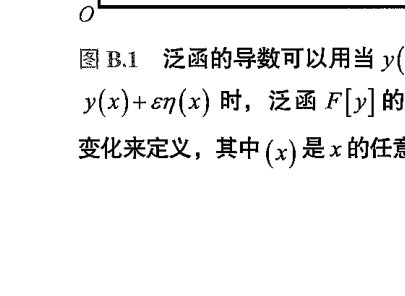
\includegraphics[width=0.7\textwidth]{appB-fig554-functional.png}
\caption{泛函的导数可以用当 $y(x)$ 变为 $y(x)+\epsilon\eta(x)$ 时，泛函 $F[y]$ 的值如何变化来定义，其中 $\eta(x)$ 是 $x$ 的任意函数。}
\label{fig:appB-functional}
\end{figure}

考虑一个定义在函数 $G(\dot{y}(x),y(x),x)$ 的积分之上的泛函，它同时还依赖于 $y(x)$ 及其导数 $\dot{y}(x)$，并且直接依赖于 $x$：
\begin{align}
F[y]=\int G(\dot{y}(x),y(x),x)\,\mathrm{d}x
\label{align:appB-functional}
\end{align}
其中，假设 $y(x)$ 的值在积分的边界处（可能在无穷大处）为定值。考虑函数 $y(x)$ 的变动，我们可以得到
\begin{align}
F[y(x)+\epsilon\eta(x)]=F[y(x)]+\epsilon\int\Big\{\frac{\partial G}{\partial y}-\frac{\mathrm{d}}{\mathrm{d}x}\Big(\frac{\partial G}{\partial \dot{y}}\Big)\Big\}\eta(x)\,\mathrm{d}x+O(\epsilon^2)
\label{align:appB-expand}
\end{align}
让我们以式~\eqref{align:appB-functional-deriv} 的形式来表示式~\eqref{align:appB-expand}。为此，对式~\eqref{align:appB-expand} 右侧的第二项进行分部积分，并注意 $\eta(x)$ 必须在积分的边界处消除（因为 $y(x)$ 在边界处为定值），从而得到
\begin{align}
F[y(x)+\epsilon\eta(x)]=F[y(x)]+\epsilon\int\frac{\delta F}{\delta y(x)}\eta(x)\,\mathrm{d}x+O(\epsilon^2)
\label{align:appB-extract}
\end{align}
与式~\eqref{align:appB-functional-deriv} 进行比较，即可确定泛函的导数。由于要求消除泛函的导数，因此有
\begin{align}
\frac{\partial G}{\partial y}-\frac{\mathrm{d}}{\mathrm{d}x}\Big(\frac{\partial G}{\partial \dot{y}}\Big)=0
\label{align:appB-euler-lagrange}
\end{align}
这就是\textbf{欧拉-拉格朗日}（Euler-Lagrange）方程。例如，如果
\begin{align}
G=\dot{y}(x)^2+y(x)^2
\end{align}
则欧拉-拉格朗日方程的形式变为
\begin{align}
y(x)-\ddot{y}(x)=0
\label{align:appB-EL-simple}
\end{align}
这个二阶微分方程可以利用 $y(x)$ 的边界条件来求解。

考虑由积分定义的泛函，其积分采用 $G(y,x)$ 的形式，并且不依赖于 $\dot{y}(x)$。在这种情况下，只要 $x$ 的所有值都满足 $\partial G/\partial y(x)=0$，就能保证解的稳定性。

如果我们关于概率分布优化一个泛函，则需要保持概率的归一化约束。满足该要求的最简单方式就是使用拉格朗日乘子（参见附录~C），其允许进行无约束的优化。

上述结果可以直接扩展到多维变量 $x$ 上。有关变分法的更全面讨论，请参阅 Sagan (1969)。

\end{document}